\chapter{交互演示与数据发布}
\label{ch:demo}

演示是这台蒸烤一体机的腔体，不是另一套传热模型。画面中央是食品，上方是加热器，蒸汽和风机是两个边界标记。积分、更新、评分和投影属于可测试的数值核；页面只读状态流。页面上的每个量和下载字段都要能指回方程。数值核尚未按规格实现的部分，本章只保留规格，并单独写下已经放进 \texttt{acts-mcdt/demo} 的页面实际做了什么。

规格中的在线模型是两节点热容网络。已运行的评分核和当前页面都是一维十六条控制体，不是多孔介质真值。两节点方程只保留在探针命题里。三者的常数、列名和时间常数不能混写。浏览器轨迹上的温度、进度或中位数不得进入主表。主表只收第 10 章日志。

\begin{figure}[ht]
\centering
\begin{tikzpicture}[
  node distance=6mm and 8mm,
  box/.style={draw, rounded corners, align=center, font=\small, inner sep=3pt, minimum width=28mm},
  arr/.style={-{Stealth}}
]
\node[box] (k) {数值核\\积分与投影};
\node[box, right=of k] (s) {状态流\\同一时刻};
\node[box, right=of s] (p) {页面四块};
\node[box, below=of k] (a) {无界面断言};
\node[box, below=of p] (d) {下载字段};
\draw[arr] (k)--(s);
\draw[arr] (s)--(p);
\draw[arr] (k)--(a);
\draw[arr] (s)--(d);
\end{tikzpicture}
\caption{演示各层的依存关系图，不是测量。页面与断言都只消费数值核已经写出的状态，不另起积分。}
\end{figure}

\section{页面必须同时露出的四块}

\paragraph{要判定的量}
一次运行是否同时露出边界、状态、路径和投影。四块缺一块，操作者就不能在同一时刻核对停止、探针是否有效、以及加热请求是否被屏障改写。要判定的不是版式是否美观，而是四个量能否指回同一时刻的状态向量。

决策状态取
\[
\vect{z}=\big(T_{\mathrm{cold}},\,\bar T_s,\,\sigma_T,\,\bar\varepsilon_l,\,\varepsilon_{l,s},\,\alpha_m,\,\alpha_b,\,S,\,\Delta m\big).
\]
冷点温度、表面均温、温度离散、平均液相、表面液相、热力进度、表面褐变、结壳和累计质量损失。页面的状态块至少要能读出其中与当前真值同构的那几项，并标明哪些项尚未进入状态流。

\paragraph{继承的文献层与不继承的层}
四块继承的是决策状态的划分、蒸汽干预的三条路径，以及屏障投影把参考动作和安全动作分开这一形式。不继承某一界面库的组件树，也不继承浏览器副本里为了画条而写的显示公式。文献里的体积平均方程、集合更新和二次投影都不是页面脚本。页面不因为画出了色带就继承那些方程的结论。

\paragraph{方程、算法或协议}
边界块露出加热、蒸汽、风速、排汽。记投影后的执行量为 $\vect{u}=(u_h,u_{\mathrm{st}},u_v,u_{\mathrm{ex}})$。策略可以写它们，操作者也可以接管。接管时段的标记为干预。路径在该时段按 $\mathrm{do}(u_{\mathrm{st}})$ 计算，把结构方程里的蒸汽节点换成接管值，不按策略与结果的条件相关计算。未接管时，蒸汽仍是策略的子节点，相关不能当成效应。

状态块露出 $T_1$、$T_2$、含水、$\alpha_m$、$R_{\mathrm{int}}$ 的后验均值和方差。真值曲线与估计曲线分开着色。评分核里表面温度是第 0 个控制体，冷点是十六条里的最低温度，估计是以时间常数跟踪表面观测的 $\widehat T_c$。两节点规格里的 $T_1,T_2$ 与这三列不是同一个离散对象。同屏时必须写明列来自哪一个积分器。

路径块露出当前蒸汽设定下的三项。品质泛函 $Q$ 只依赖进度和表面含水，进度只通过内部温度依赖蒸汽，内部温度对蒸汽的依赖再分成热阻固定与热阻随结壳变化。链式法则给出
\begin{align*}
\frac{\mathrm{d}Q}{\mathrm{d}m_{\mathrm{st}}}
&=
\underbrace{\frac{\partial Q}{\partial\alpha_m}\frac{\partial\alpha_m}{\partial T_2}\frac{\partial T_2}{\partial q_{\mathrm{lat}}}}_{\mathrm{A}}
+
\underbrace{\frac{\partial Q}{\partial\varepsilon_{l,s}}\frac{\partial\varepsilon_{l,s}}{\partial m_{\mathrm{st}}}}_{\mathrm{B}}
+
\underbrace{\frac{\partial Q}{\partial\alpha_m}\frac{\partial\alpha_m}{\partial T_2}\frac{\partial T_2}{\partial R_{\mathrm{int}}}\frac{\partial R_{\mathrm{int}}}{\partial S}\frac{\partial S}{\partial\varepsilon_{l,s}}}_{\mathrm{C}}.
\end{align*}
A 是潜热到冷点，B 是表面水分到品质，C 是结壳到内部热阻再到冷点。符号在抽样中不稳定时只留区间，不把样本均值的符号画成确定结论。短窗口内 C 相对 A 是 $O(\tau/\tau_S)$，全时域才保留完整长度。

投影块同时露出品质模块请求的加热量 $u_{\mathrm{req}}$ 和进入边界的加热量 $u_h$。管温贴近 $h_T=0$ 时二者必须分开，否则屏障是否动作在页面上不可见。规格中的屏障自变量只有漏电、水位或干烧、加热器温度、腔压和门。后验可以移动参考点，不能移动可行域。

策略四档与试验章相同：开环、腔温闭环、无探针优化、对偶控制。可改的样品因素是厚度档、初始温度、初始含水和种子。

已经放进页面的实现与上述规格不一致，必须分开记账。策略下拉有开环、腔温比例、无探针和对偶四档。操作者能改的只有厚度、时间索引和切面位置。种子固定为 7，初温固定为 $8^\circ\mathrm{C}$，含水固定为 0.72，原型固定为肉糜，非均质固定为均匀。页面分成控制、场景读数和本帧读数三栏，不是四块等权区域。边界执行量没有接管开关。状态区同时写出表面、冷点、估计、选中控制体和进度。估计列存在，真值与估计没有分成两种颜色，也没有后验方差带。第三栏写出加热请求、加热指令、蒸汽、风机、热阻方差、加热器温度、表面活度和结壳。没有按链式法则画出的路径条，也没有
\[
A=0.4\,u_{\mathrm{st}}+0.15,\qquad
B=-0.25\,u_{\mathrm{st}},\qquad
C=-0.1\,(1-\mathrm{Var})
\]
这种显示公式。投影区用两行数字给出请求和指令，场景里没有两根针。

\paragraph{本节不能推出的结论}
四块同时出现只说明规格要求同屏核对。当前页面没有四块的全部对象，不能推出演示已经满足规格。侧栏数字不是路径 A、B、C 的估计，不能写入结果句。页面上读到的温度不能进入主表。

\section{页面上的机制，而不是说明文字}

\paragraph{要判定的量}
操作者不读旁注，能否从图形本身核对两件事：探针无效时停止标记不动；长时间只维持腔温时，内部热阻的方差保持为先验。厚度超过信息上限时，要判定的是剩余时间是否被改成区间，而不是是否给出一个看起来精确的分钟数。

\paragraph{继承的文献层与不继承的层}
继承的是信息动作为一次可执行实验、以及稳态平衡观测对内部热阻灵敏度为零这两层问题提法。不继承最优实验设计的离线一次性设计，也不继承“说明文字可以把缺失的图形补上”。机制必须由色带、标记和区间本身承担。装饰动画不继承任何状态方程。

\paragraph{方程、算法或协议}
默认视图把 P4 画成两段色带，叠在 $T_1$ 与 $R_{\mathrm{int}}$ 方差上。第一段使界面相变变号，第二段只改外部热阻。评分核里对偶策略的探针窗口是
\[
t\in[150,190)\ \mathrm{s},\qquad \mathrm{Var}(r)>0.25,\qquad \text{未锁定}.
\]
$170\,\mathrm{s}$ 之前蒸汽指令为 $1$，其后风速为 $1.3$，窗口外风速回到 $0.4$。$190\,\mathrm{s}$ 之后才允许更新内部热阻估计
\[
r_{\mathrm{new}}=\mathrm{clip}\big(1.4+1.1\,\ell+1.2\,(L/0.03),\,0.8,\,7\big),
\]
其中滞后被限制在 $\ell=\mathrm{clip}((y_T-\widehat T_c)/6,\,0,\,3)$。仅当 $r_{\mathrm{new}}$ 比当前估计更接近热阻代理 $r_{\mathrm{proxy}}$ 时，才把估计换成 $r_{\mathrm{new}}$，并把方差乘 $0.35$。方差不降的运行，停止标记保持在动作前的位置。这是无效探针的页面核对，不是一句提示语。

稳态开关的规格是：长时间内只维持腔温，质量变化与潜热为零。两节点平衡迫使 $T_1=T_2=T_\infty$，对 $R_{\mathrm{int}}$ 求导后右端仍为零，页面上该方差保持为先验。评分核上的数值核对是三组热阻的平衡温度极差为 $0$。页面没有这个开关，也没有把方差画成色带。

厚度拨到信息上限以外时，剩余时间的位置改成区间。信息上限来自被动观测的秩，不来自界面上的滑块刻度。当前页面的时间滑块始终给出一个时刻，没有区间显示。

页面对偶探针与评分核使用同一窗口和同一乘子。窗口是 $[150,190)$ 且方差大于 $0.25$。$170\,\mathrm{s}$ 之前蒸汽为 1，其后风机为 1.3。$190\,\mathrm{s}$ 之后才计算
\[
r_{\mathrm{new}}=\mathrm{clip}\big(1.4+1.1\,\ell+1.2\,(L/0.03),\,0.8,\,7\big),
\]
并且只在更接近 $r_{\mathrm{proxy}}$ 时替换估计、把方差乘 $0.35$。评分核把 \texttt{probe\_locked} 初始化为假，循环里没有把它写成真，窗口结束靠时刻离开 $[150,190)$。\texttt{probed} 在更新之后写成真，用来阻止第二次更新。页面把同一个 \texttt{probed} 放进窗口条件。两边都只更新一次。默认时长 55 min，开环会在菜单终点把加热写成 0。页面第三栏能读出方差和加热请求，没有单独的“停止标记留在动作之前”的图形。因此无效探针否决在页面上只能从数字读，不能从色带读。演示规格里的色带仍是规格，不能把侧栏数字说成已经画出两段探针。

\paragraph{本节不能推出的结论}
侧栏里的方差数字不等于 P4 的两列灵敏度线性无关。那条秩命题的数值是表面—内部滞后 $40.846$ 与单独蒸汽 $38.912$，判据是差值大于 $1$，不是 $1.15$ 倍。该核对属于无界面断言，不属于页面。页面里方差乘 $0.35$ 不能推出探针有效，也不能移动主表里的停止时刻。

\section{下载字段}

\paragraph{要判定的量}
一次运行能否被另一门语言逐列重算。要判定的是字段是否固定、参数文件里的数是否就是积分用的数，以及浏览器导出的表是否与评分核的表为同一对象。

\paragraph{继承的文献层与不继承的层}
继承的是可重复试验对输入输出的合同：同一常数、同一噪声、同一初始条件必须得到同一轨迹。不继承界面状态管理器的内部结构，不继承为了展示而四舍五入之后另存的一套参数。科学数据格式的习惯只提供“一行一个时刻”这一层，不提供列名的物理含义。

\paragraph{方程、算法或协议}
规格要求一次运行三个文件。

\begin{table}[ht]
\centering
\caption{规格中的下载字段}
\begin{tabularx}{\textwidth}{llX}
\toprule
文件 & 行或键 & 必须含有 \\
\midrule
\texttt{trajectory.csv} & 每个时间步一行 & $t,T_1,T_2,\hat T_2,m,\alpha_m,R_{\mathrm{int}},\mathrm{Var},u,u_{\mathrm{proj}},\mathrm{mode}$ \\
\texttt{summary.json} & 一次运行 & 停止时刻、$e_{\alpha}$、能量、A、B、C、探针是否有效 \\
\texttt{parameters.json} & 一次运行 & 两节点常数、噪声、种子、策略名、是否同构真值 \\
\bottomrule
\end{tabularx}
\end{table}

\texttt{mode} 的取值是品质、信息、保温、干预。参数文件中的热容、热阻、潜热系数、噪声幅度和种子必须是积分器读入的那一组。展示用副本若改了单位或截断了小数，就不能再当作参数文件。

评分核的战役摘要比该规格少了路径 A、B、C 和同构标记。页面导出的表头是
\[
\texttt{time,t\_surf,t\_core,t\_hat,heat,heat\_req,steam,var\_r,heater,alpha\_m,mode}.
\]
十一列。步长 \(2\,\mathrm{s}\)，每四步记一行，间隔 \(8\,\mathrm{s}\)，默认时长 55 min，与种子 7 的 Python 轨迹相同，共 414 行。导出里有估计、加热器和模式。没有平均含水，没有风速，没有 \texttt{summary.json}，没有 \texttt{parameters.json}。\(\texttt{t\_core}\) 是十六条里更新前的最低温度，\(\texttt{t\_hat}\) 才是估计。两列都在，不能把冷点列当成估计。

Python 的 \texttt{demo\_seed7\_dual.csv} 有平均含水，没有加热器。两边共有的表面、冷点和估计，在种子 7、肉糜、30 mm、初温 \(8^\circ\mathrm{C}\)、含水 0.72、对偶策略上，最大差低于 \(5\times 10^{-6}\,\mathrm{K}\)。差来自 CSV 保留五位小数。含水列和加热器列没有这一条逐列身份。浏览器上改过厚度或策略之后的导出，没有再和 Python 对过。

能量若从浏览器的加热列重算，得到的是指令乘 \(8\,\mathrm{s}\) 的展示和。规格中的 \(e_\alpha\) 是停止时刻的 \(\alpha_m-0.85\)。\(0.85\) 是设计量。进度饱和到 1 之后，\(e_\alpha\) 的上沿是 \(+0.15\)。这些定义属于评分核的停止样本。主表仍只引用第 10 章。

\paragraph{本节不能推出的结论}
下载按钮存在不等于字段合同已经满足。十一列文件没有路径增益，也没有同构真值标记。三列温度对齐不能写成全部字段已经和战役日志一致。

\section{计算与界面分开}

\paragraph{要判定的量}
积分、断言、界面和离线真值是否分属四层，以及界面有没有为了画面改方程。要判定的还包括：浏览器里的步进是评分核的十六条格式，还是另一套方程。

\paragraph{继承的文献层与不继承的层}
继承的是估计与真值隔离、以及断言不依赖点击这一试验合同。不继承“同一种语言写出来的脚本就是同一个模型”。评分核用数组积分；页面用另一段脚本来画。语言相同不能合并这两层。着色器只继承已经算出的数组，不继承传热方程。

\paragraph{方程、算法或协议}
四层的合同如下。

\begin{table}[ht]
\centering
\caption{计算与界面的分层}
\begin{tabularx}{\textwidth}{lXX}
\toprule
层 & 职责 & 不允许的越界 \\
\midrule
数值核 & 真值、噪声、更新、探针评分、路径、投影 & 为了画面平滑而改方程 \\
断言 & 稳态、两段脉冲、冷点上界、屏障的可重复检查 & 依赖界面点击才成立 \\
界面 & 四块、色带、区间、下载 & 自行积分或另存一套参数 \\
离线真值 & 多孔介质、等温线、各向异性、脂肪夹层、收缩 & 改列名后再进界面 \\
\bottomrule
\end{tabularx}
\end{table}

评分核的常数是 $\alpha=2.0\times 10^{-7}\,\mathrm{m^2/s}$，$\rho c=3.4\times 10^{6}\,\mathrm{J/(m^3\,K)}$，模块级潜热 $2.3\times 10^{6}\,\mathrm{J/kg}$，空间步长为厚度的 $1/16$。由此均匀导热率为
\[
k=\alpha\rho c=2.0\times 10^{-7}\times 3.4\times 10^{6}=0.68\,\mathrm{W/(m\cdot K)}.
\]
潜热常数在战役步进里没有乘到质量流上。边界通量写成
\[
q=h(T_\infty-T_s)+q_{\mathrm{lat}}+7000\,u_h,
\]
其中 $h=12+55\,u_v$，$T_\infty=90+95\,u_h$，而
\[
q_{\mathrm{lat}}=18000\,u_{\mathrm{st}}(1-a_w)-9000\,(1-u_{\mathrm{st}})\max(a_w-0.35,0)\,u_v.
\]
这是经验通量，不是 $\Delta h\cdot\dot m$。水分扩散系数 $2\times 10^{-9}\,\mathrm{m^2/s}$，再乘 $(1+3m)$。进度在冷点上
\[
\dot f=10^{(T_{\mathrm{core}}-70)/10}/60,\qquad \alpha_m=1-\exp(-f/2),
\]
只在实现中作为饱和映射，不是把全部品质写成一级反应。噪声是确定性正弦散列，温度幅度 $0.4^\circ\mathrm{C}$，含水幅度 $0.004$，没有随机数发生器。种子为 $1000+\mathrm{seed}+17\times(\text{原型编号})$。\texttt{hetero}=2 把下标 $5$ 的控制体导热降到 $0.45$ 倍；\texttt{hetero}=1 给空间温度 $\pm 4^\circ\mathrm{C}$。战役时长 $55$ 分钟，步长 $2\,\mathrm{s}$。

表面控制体的通量项可以化成与一条切片热容相同的系数。扩散率除以导热率等于 $1/(\rho c)$，空间步长 $L/16$，于是通量对表面温度的贡献为
\[
\Delta T_s=\Delta t\cdot q\cdot\frac{16}{\rho c\, L}.
\]
内部点仍由十六条的离散二阶差分推进，脂肪夹层只改其中一个控制体的扩散率。

页面脚本使用同一格式。控制体数是 16。潜热通量使用上面的 $q_{\mathrm{lat}}$，含活度，也含无蒸汽时的蒸发项。内部点是二阶差分，不是集总时间常数。$L=0.03\,\mathrm{m}$ 时扩散时间
\[
L^2/\alpha=9\times 10^{-4}/(2.0\times 10^{-7})=4500\,\mathrm{s}.
\]
页面没有另一套 $\tau_2=180\,(L/0.03)^2$ 的内部节点。

观测器也在页面里积分。对偶与无探针两支都用
\[
\tau=\mathrm{clip}(\hat r,0.8,8)\,(L/0.03)^2\cdot 280,
\]
先验 $\hat r=5$、$L=0.03\,\mathrm{m}$ 时 $\tau=1400\,\mathrm{s}$。估计被压到表面观测之下至少 $4\max(\hat r-1,0.2)$。先验为 $5$ 时，这条下压是 $16\,\mathrm{K}$。种子 7 的第一步因此把估计放到约 $-7.9^\circ\mathrm{C}$，而冷点仍是 $8^\circ\mathrm{C}$。加热请求
\[
u_{\mathrm{req}}=\mathrm{clip}\big(0.35+(75+m_g-\widehat T_c)/30,\,0.15,\,1\big),
\]
裕量 $m_g=6+10\sqrt{\mathrm{Var}}\,(L/0.03)$。方差取先验 $0.64$ 时 $\sqrt{\mathrm{Var}}=0.8$，厚度 $0.03\,\mathrm{m}$ 的裕量是 $14\,\mathrm{K}$，等效目标是 $89^\circ\mathrm{C}$。请求看见的是估计，不是把真节点直接送进代数式。

停止规则与评分核相同。估计超过 $75+m_g$ 且时刻晚于 $240\,\mathrm{s}$ 才允许停。对偶、方差仍大于 $0.45$ 且厚度大于 $0.04\,\mathrm{m}$ 时否决停止。开环菜单时间是 $900+18000(L-0.015)$，单位为秒。默认时长是 55 min。厚度 $0.05\,\mathrm{m}$ 的菜单时间 $1530\,\mathrm{s}$ 落在这个窗口内，开环会走到菜单终点。

加热器两边都用
\[
\Delta T_h=\Delta t\big(0.015\,u_{\mathrm{req}}(280-T_h)-0.008(T_h-40)\big).
\]
评分核和页面都在 $T_h>230^\circ\mathrm{C}$ 后按 $(T_h-230)/40$ 削减请求，最多削减 $75\%$。断言用的屏障测试函数是另一条：加热器超过 $210^\circ\mathrm{C}$ 时把请求剪到 $0.25$，并且不随后验改变。物理削减从 $230^\circ\mathrm{C}$ 开始。两处阈值不同。页面若只画出 $230^\circ\mathrm{C}$ 的削减，不能代替 $210^\circ\mathrm{C}$ 的测试函数。满功率平衡约 $196.5^\circ\mathrm{C}$，两条阈值在这条常微分方程上都不动作。

无界面断言先于三维视图。已记录的核对是：稳态极差 $0$；两段脉冲滞后 $40.846$，单独蒸汽 $38.912$，差值大于 $1$；冷点上界 $1.2$，离散实现 $1.143$；屏障测试函数在两个不同后验下都剪到 $0.25$。这些数来自断言，不来自浏览器。

界面规格要求机制视图与仿真视图使用同一时刻的状态。机制视图的线的明暗由偏效应或方差决定。仿真视图的几何按厚度与收缩显示。当前页面的三维对象读的是这段十六条脚本返回的场，不是多孔介质真值。着色器只设置颜色和自发光，不在片元里积分第二套方程。

热阻更新仍使用真温度差构造的 $r_{\mathrm{proxy}}$。页面与评分核在这一点上相同，所以三列温度对齐不能把估计写成只读观测的滤波器。

日志里每个策略 $4860$ 条，四策略合计 $19440$ 条。该条数与 $1620\times 4$ 不一致。未按同一脚本重跑并核对行数之前，不把 $1620$ 当作日志条数。$19440$ 条是同一数值过程的样本，不是独立实验。主对照的中位数只引用第 10 章：开环 $e_\alpha$ 为 $-0.8425$、提前比例 $0.6667$、能量 $1170$；腔温闭环为 $0.15$、$0.2222$、$3310$；无探针优化为 $-0.4666$、$0.9444$、$1655.2$；对偶为 $-0.3127$、$0.9019$、$1729.7$。负值表示停在设计线之下。

\paragraph{本节不能推出的结论}
表面、冷点和估计三列对齐，不能推出含水、风速、路径增益或同构真值也已对齐。断言通过只说明四条判据的方向。多孔介质真值、集合更新和求解器都还不是这次页面背后的积分器。热阻更新仍读真温度差。加热器削减在这条平衡上不动作。排汽没有标记。路径三项没有长度。页面因此不是规格中的完整演示。

\section{三维场景里必须能读出的量}

\paragraph{要判定的量}
每个可见元素能否对应一个状态分量。要读出的是厚度坐标上的温度或进度、投影后的四个边界强度、探针所在的时间段、三条路径的偏效应，以及请求加热与投影加热是否分开。相机只能帮助读这些量，不能提供与状态无关的漫游。

\paragraph{继承的文献层与不继承的层}
继承的是“冷点可以不在几何中心”这一现象层，以及切面必须来自已经算出的场。不继承腔体效果图的布光和材质习惯。不继承在着色器里再解一遍热方程。两节点阶段必须标明插值；没有脂肪层的日志不得画出脂肪层。

\paragraph{方程、算法或协议}
规格中的食品实体按 $L(t)$ 缩放。切面滑块给出厚度坐标 $s\in[0,1]$ 上的 $T$、$\varepsilon_l$ 或 $\alpha$，色标固定在该次运行的最小与最大，不随帧重归一化到全色。两节点阶段的切面由表面节点与内部节点插值，并标明“两节点插值”。多孔介质日志接入后改用空间列。T2 日志含脂肪夹层时才显示独立薄层。四个边界标记的强度等于投影后的 $\vect{u}$，不是请求值。探针两段在时间轴上着色，并在表面闪动一次；闪动不改变几何。路径条的长度是偏效应，符号不稳定时改为中性色并标区间。请求与投影分成两根针，重合表示屏障未动作。相机只提供旋转、缩放和切面。

预置应包含主对照的一个种子、一次遮挡、一次屏障贴近，以及一维与二维各一条同名种子。操作者可改策略并重算两节点。多孔介质条目从日志载入，不在浏览器内重解偏微分方程。

页面现在使用与评分核相同的十六条显式格式。种子 7、肉糜、30 mm、初温 $8^\circ\mathrm{C}$、含水 0.72、对偶策略下，表面、冷点和估计与 \texttt{demo\_seed7\_dual.csv} 的最大差都低于 $5\times 10^{-6}\,\mathrm{K}$。差来自 CSV 保留五位小数。冷点按日志的顺序取值：导热更新之前的最低温度。色标固定在 $5^\circ\mathrm{C}$ 到 $170^\circ\mathrm{C}$，不随帧重归一化。十六块并排，颜色是该控制体的温度。横向尺度按 \(L/0.03\) 缩放，厚度滑块改变 \(L\) 之后重新积分，盒子随之变窄或变宽。下方色条是同一组数的平面读法，黑框标出选中的控制体。指针拖动绕食品旋转，滚轮改变距离。没有与状态无关的漫游。

\begin{figure}[ht]
\centering
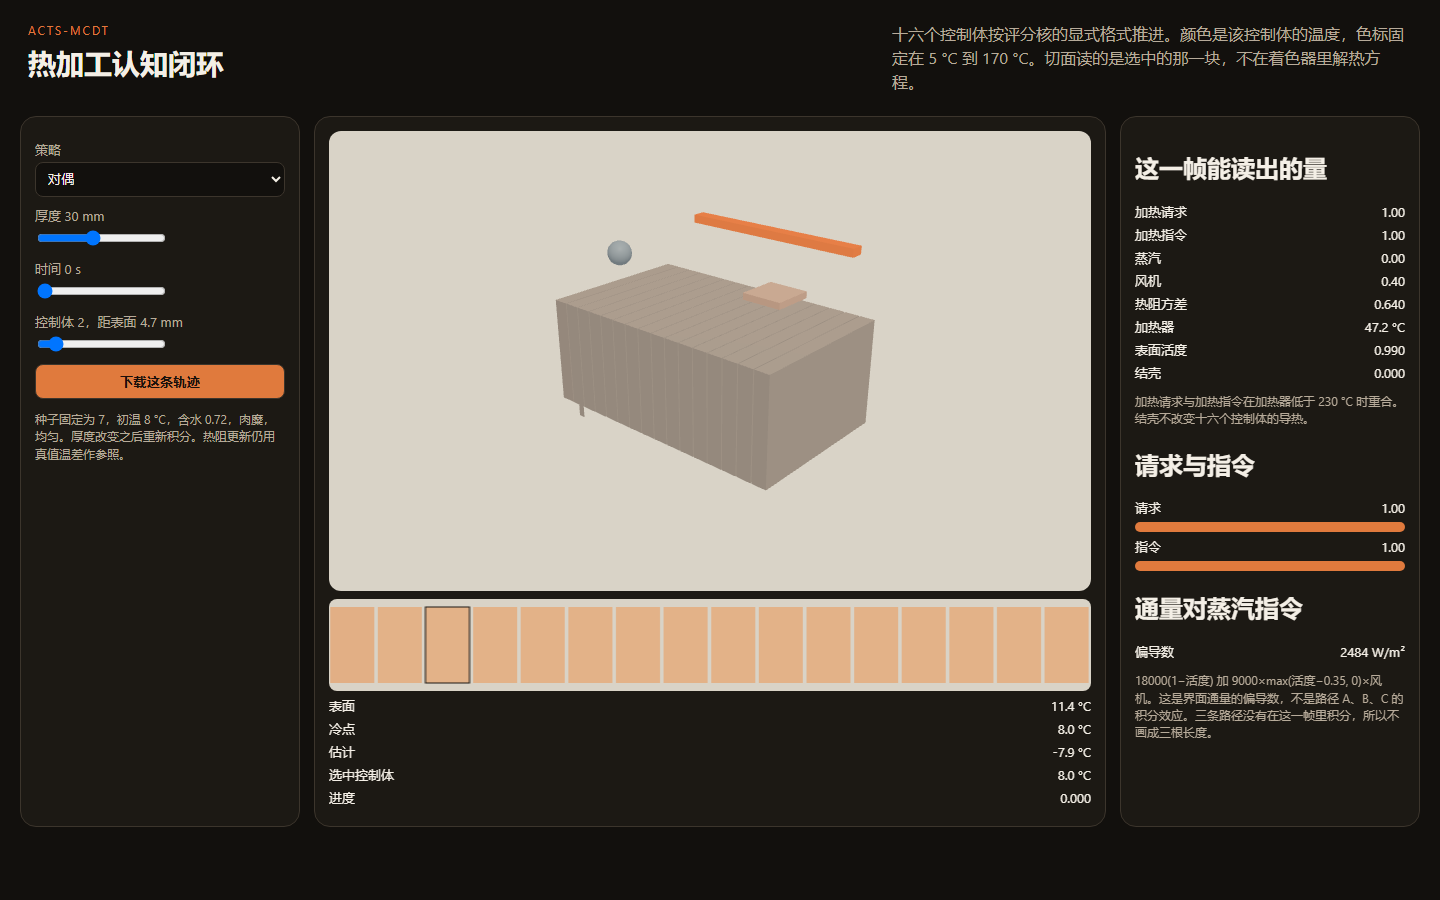
\includegraphics[width=\textwidth]{paper/E_demo_start.png}
\caption{同一条轨迹的起点。表面 $11.4^\circ\mathrm{C}$，冷点 $8.0^\circ\mathrm{C}$，估计 $-7.9^\circ\mathrm{C}$。估计为负，是表面读数减去 16 K 的上限，不是传感器读数。十六块颜色接近，因为场还没有拉开。}
\end{figure}

\begin{figure}[ht]
\centering
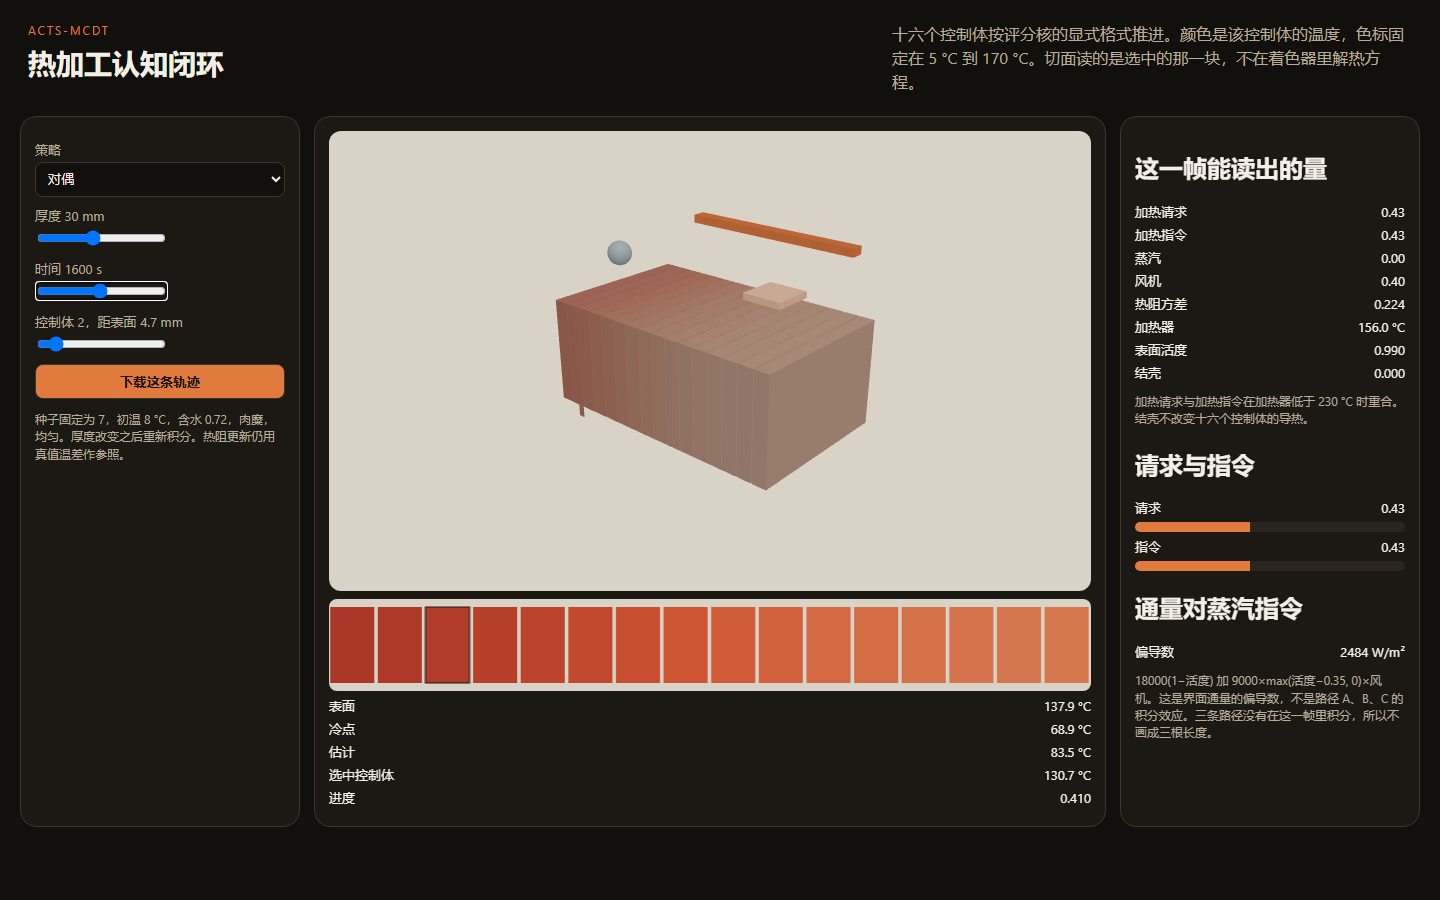
\includegraphics[width=\textwidth]{paper/E_demo_late.png}
\caption{1600 s。表面 $137.9^\circ\mathrm{C}$，冷点 $68.9^\circ\mathrm{C}$，估计 $83.5^\circ\mathrm{C}$，进度 0.410，方差已经是 0.224。色条从表面到深处由深变浅。加热请求与加热指令都是 0.43，加热器 $156^\circ\mathrm{C}$，削减没有动作。}
\end{figure}

加热器是一根细盒子。自发光强度是 $0.08+0.9\,u_h$，随投影后的加热变化，不随请求变化。蒸汽是一颗球，自发光随投影后的蒸汽指令。风机是一块扁盒，自发光随投影后的风机除以 1.3。核里没有单独的排汽状态，所以不设第四个标记。150 s 至 190 s 内，最靠近表面的一块控制体自发光，几何不变。侧栏有请求和指令两根针；加热器低于 \(230^\circ\mathrm{C}\) 时两者重合。同一栏写出通量对蒸汽指令的偏导数 \(18000(1-a_w)+9000\max(a_w-0.35,0)\,u_v\)。路径 A、B、C 没有积分，不把这个导数画成三根长度。切面仍是十六条里被选中的那一块，不是表面与冷点的插值。没有脂肪层开关。

遮挡预置、屏障贴近预置、以及同一种子的一维与二维并置，都还没有放进页面。同一种子的二维轨迹本身也还没有作为预置文件生成。因此当前三维场景不能用来核对遮挡后的探针有效率，也不能用来核对脂肪层是否改变冷点位置。

着色器不积分第二套方程：每一帧只改已有材质的颜色和自发光，再画一次。传热发生在页面脚本的十六条控制体里。该格式与评分核相同，种子 7 的三列温度差低于 \(5\times 10^{-6}\,\mathrm{K}\)。它仍不是多孔介质真值，颜色也不能称为第 10 章主结果的场。主结果只引用战役日志。

\paragraph{本节不能推出的结论}
画面中有盒子、切面和发热条，不能推出冷点位置、探针时序或屏障动作已经被读出。固定色相窗不是运行内的固定色标。没有轨道和缩放，不能把规格中的相机写成已经提供。未接入的预置不能在演示里当成已经核对的病例。
